\subchapter{Board setup}{Objective: setup communication
with the board and configure the bootloader.}

After this lab, you will be able to:
\begin{itemize}
\item Access the board through its serial line.
\item Configure the U-boot bootloader and a tftp server
      on your workstation to download files through tftp.
\end{itemize}

\section{Getting familiar with the board}

Take some time to read about the board features and connectors:

\begin{itemize}
   \item If you have the original BeagleBone Black:\\
         \url{https://www.elinux.org/Beagleboard:BeagleBoneBlack}
   \item If you have the newer BeagleBone Black Wireless:\\
	 \url{https://www.beagleboard.org/boards/beaglebone-black-wireless}
         in addition to the above URL.
\end{itemize}

Don't hesitate to share your questions with the instructor.

\section{Download technical documentation}

We are going to download documents which we will need during our
practical labs.

The first document to download is the BeagleBone Black System Reference Manual found at
\url{https://github.com/CircuitCo/BeagleBone-Black/blob/master/BBB_SRM.pdf?raw=true}.

Even if you have the BeagleBoneBlack Wireless board, this is the
ultimate reference about the board, in particular for the pinout and
possible configurations of the P8 and P9 headers, and more generally
for most devices which are the same in both boards.
You don't have to start reading this document now but you will need it
during the practical labs.

The second document to download is the datasheet for the
TI AM335x SoCs, available on
\url{https://www.ti.com/lit/ds/symlink/am3359.pdf}. This document will
give us details about pin assignments.

Last but not least, download the Technical Reference Manual (TRM) for
the TI AM3359 SoC, available on \url{https://www.ti.com/product/am3359},
in the \code{User guides} section in the \code{Technical documents} tab.
This document is more than 5100 pages big! You will need it
too during the practical labs.

\section{Setting up serial communication with the board}

The Beaglebone serial connector is exported on the 6 pins close to one
of the 48 pins headers. Using your special USB to Serial adapter provided
by your instructor, connect the ground wire (blue) to the pin closest
to the power supply connector (let's call it pin 1), and the \code{TX} (red)
and \code{RX} (green) wires to the pins 4 (board \code{RX}) and
5 (board \code{TX})\footnote{See
\url{https://www.olimex.com/Products/Components/Cables/USB-Serial-Cable/USB-Serial-Cable-F/}
for details about the USB to Serial adapter that we are using.}.

You always should make sure that you connect the \code{TX} pin of the cable
to the \code{RX} pin of the board, and vice versa, whatever the board and
cables that you use.

\begin{center}
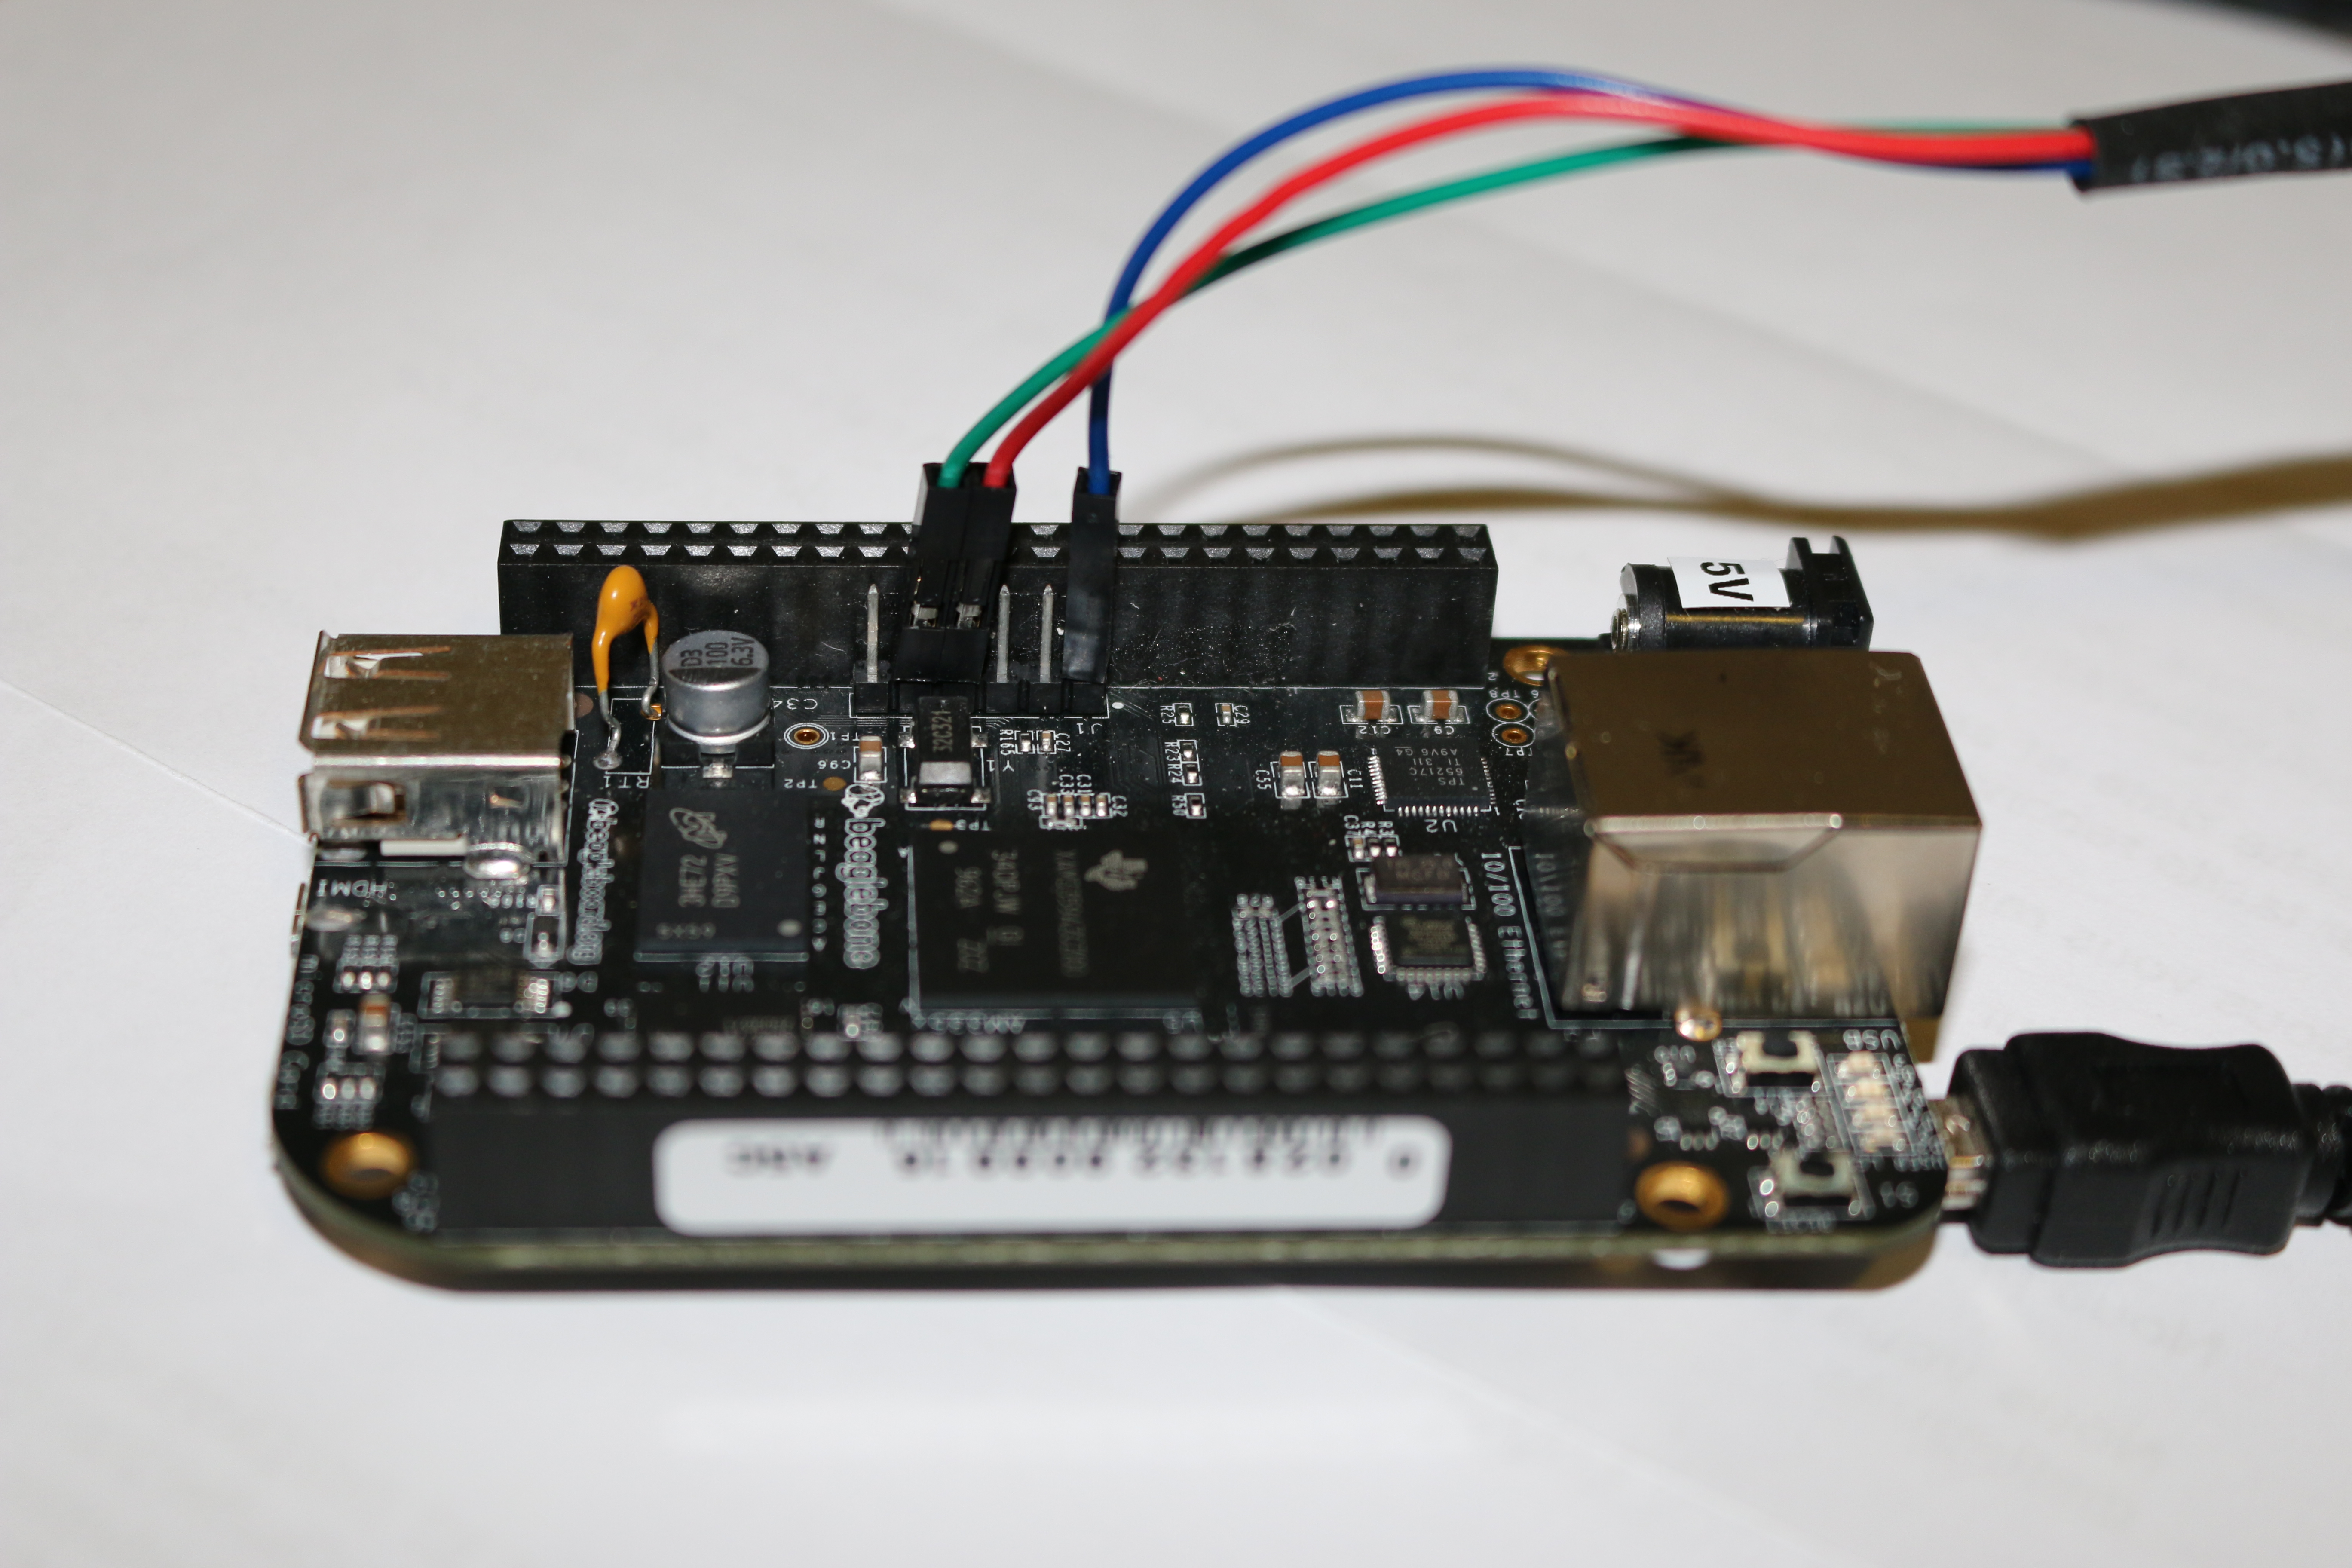
\includegraphics[width=8cm]{common/beaglebone-black-serial-connection.jpg}
\end{center}

Once the USB to Serial connector is plugged in, a new serial port
should appear: \code{/dev/ttyUSB0}.  You can also see this device
appear by looking at the output of \code{dmesg}.

To communicate with the board through the serial port, install a
serial communication program, such as \code{picocom}:

\begin{verbatim}
sudo apt install picocom
\end{verbatim}

If you run \code{ls -l /dev/ttyUSB0}, you can also see that only
\code{root} and users belonging to the \code{dialout} group have
read and write access to this file. Therefore, you need to add your user
to the \code{dialout} group:

\begin{verbatim}
sudo adduser $USER dialout
\end{verbatim}

{\bf Important}: for the group change to be effective, you have to
{\em completely log out} from your session and log in again (no need to
reboot). A workaround is to run \code{newgrp dialout}, but it is not global.
You have to run it in each terminal.

Now, you can run \code{picocom -b 115200 /dev/ttyUSB0}, to start serial
communication on \code{/dev/ttyUSB0}, with a baudrate of \code{115200}. If
you wish to exit \code{picocom}, press \code{[Ctrl][a]} followed by
\code{[Ctrl][x]}.

There should be nothing on the serial line so far, as the board is not
powered up yet.

It is now time to power up your board by plugging in the mini-USB
(BeagleBone Black case) or micro-USB (BeagleBone Black Wireless case)
cable supplied by your instructor to your PC.

See what messages you get on the serial line. You should see U-boot
start on the serial line.

\section{Bootloader interaction}

Reset your board. Press the space bar in the \code{picocom} terminal
to stop the U-boot countdown. You should then see the U-Boot prompt:

\begin{verbatim}
=>
\end{verbatim}

You can now use U-Boot. Run the \code{help} command to see the available
commands.

Type the \code{help saveenv} command to make sure that the
\code{saveenv} command exists. We use it in these labs to
save your U-Boot environment settings to the boards' eMMC storage.
Some earlier versions do not support this.

If you don't have this U-Boot prompt, it's probably because you are doing these labs on your own
(i.e. without participating to a Bootlin course), we ask you to install the U-Boot binary
that we compiled and tested. See instructions at
\url{https://github.com/bootlin/training-materials/tree/master/lab-data/common/bootloader/beaglebone-black}
for a simple way to do this.

To avoid trouble because of settings applied in previous practical labs,
we advise you to clear the U-Boot environment variables:

\begin{verbatim}
env default -f -a
saveenv
\end{verbatim}

\section{Setting up networking}

The next step is to configure U-boot and your workstation to let your
board download files, such as the kernel image and Device Tree Binary
(DTB), using the TFTP protocol through a network connection.

As this course supports both the BeagleBone Black and BeagleBone Black
Wireless boards, we're keeping things simple by using Ethernet over USB
device as this works for both boards (as the Wireless board has no
native Ethernet port). So, networking will work through the USB device
cable that is already used to power up the board.

{\bf Caution}: For the following to work, make sure that your board
is powered by a USB port on your PC. Otherwise, networking over USB
cannot work.

\section{Network configuration on the target}
Now, let's configure networking in U-Boot:

\begin{itemize}
  \item \code{ipaddr}: IP address of the board
  \item \code{serverip}: IP address of the PC host
\end{itemize}

\begin{verbatim}
setenv ipaddr 192.168.0.100
setenv serverip 192.168.0.1
\end{verbatim}

Of course, make sure that this address belongs to a separate network
segment from the one of the main company network.

We also need to configure Ethernet over USB device:
\begin{itemize}
  \item \code{ethprime}: controls which interface gets used first
  \item \code{usbnet_devaddr}: MAC address on the device side
  \item \code{usbnet_hostaddr}: MAC address on the host side  
\end{itemize}

\begin{verbatim}
setenv ethprime usb_ether
setenv usbnet_devaddr f8:dc:7a:00:00:02
setenv usbnet_hostaddr f8:dc:7a:00:00:01
\end{verbatim}

Save these settings to the eMMC storage on the board\footnote{
The U-boot environment settings are stored in some free space
between the master boot record (512 bytes, containing the partition
tables and other stuff), and the beginning of the first partition (often
at \code{32256}). This is why you won't find any related file in the
first partition of the eMMC storage.}:

\begin{verbatim}
saveenv
\end{verbatim}

\section{Network configuration on the PC host}

To configure your network interface on the workstation side, we need
to know the name of the network interface connected to your board.

Note that when the board is sitting at the U-Boot prompt, no network
interface will show up on the workstation side. It is only when U-Boot
is actively executing a network-related command (such as \code{ping}
or \code{tftp}) that it brings up the USB network connection.

From the board, run \code{ping 192.168.0.1}, and while the \code{ping}
command is running, you should see on your workstation a new network
interface named \code{enx<macaddr>}. Given the value we gave to
\code{usbnet_hostaddr}, it will therefore be
\code{enxf8dc7a000001}. Note that pinging the board from your PC will
not work: when U-Boot is sitting at its prompt, it is not able to
reply to ping requests.

Then, instead of configuring the host IP address from NetworkManager's
graphical interface, let's do it through its command line interface,
which is so much easier to use:

\begin{verbatim}
nmcli con add type ethernet ifname enxf8dc7a000001 ip4 192.168.0.1/24 +ipv4.routes "192.168.0.100"
\end{verbatim}

\section{Setting up the TFTP server}

Let's install a TFTP server on your development workstation:

\begin{verbatim}
sudo apt install tftpd-hpa
\end{verbatim}

Once the package is installed, view the contents of
\code{/etc/default/tftpd-hpa}, and check what the TFTP server home directory
(\code{TFTP_DIRECTORY} setting). If \code{/srv} exists on your system,
it should be \code{/srv/tftp}, otherwise \code{/var/lib/tftpboot/}.

If you wish to make a change to this file, you will have to restart the TFTP server:

\begin{verbatim}
sudo /etc/init.d/tftpd-hpa restart
\end{verbatim}

\section{Testing the network connection}

You can then test the TFTP connection.  First, put a small text
file in TFTP server home directory. Then, from U-Boot, do:

\begin{verbatim}
tftp 0x81000000 textfile.txt
\end{verbatim}

The \code{tftp} command should have downloaded the
\code{textfile.txt} file from your development workstation into the
board's memory at location \code{0x81000000} (this location is part of
the board DRAM). You can verify that the download was successful by
dumping the contents of the memory:

\begin{verbatim}
md 0x81000000
\end{verbatim}

We are now ready to load and boot a Linux kernel!
